\chapter{Stability Photos}\label{ch:appendixB}

\begin{figure}[htbp]
    \centering
    % Second row
    \begin{subfigure}[t]{0.5\textwidth}
        \centering
        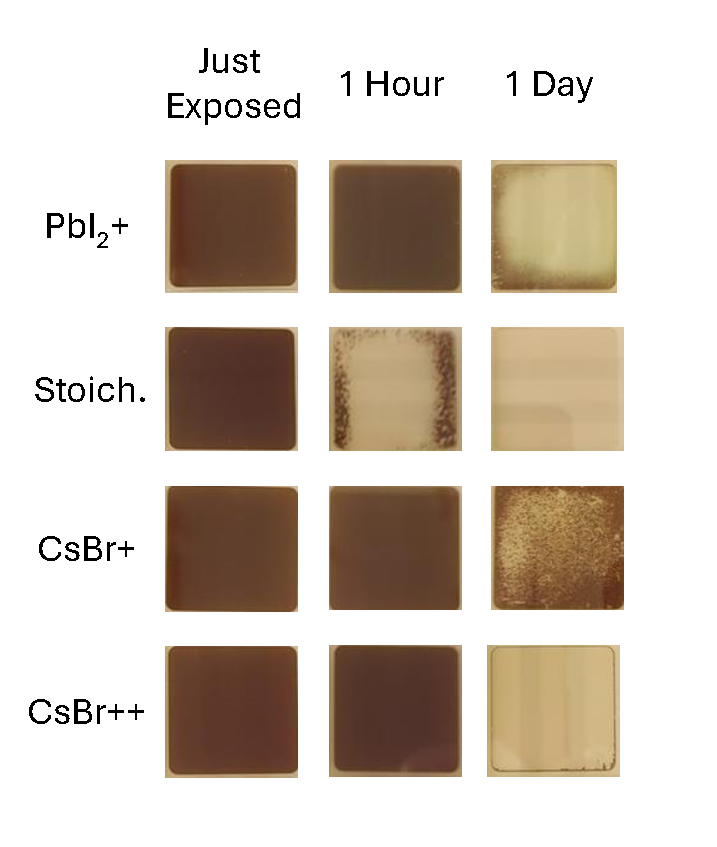
\includegraphics[width=\textwidth]{chapters/appendixB/images/Stability_Rotation_Stoichiometries_v2.pdf} % Replace with your image file
             
    \end{subfigure}

    \caption{Second set of samples}
    \label{fig:appendix:stoichiometry_rotation_V2}
\end{figure}


\begin{figure}[htbp]
    \centering
    % Second row
    \begin{subfigure}[t]{0.99\textwidth}
        \centering
        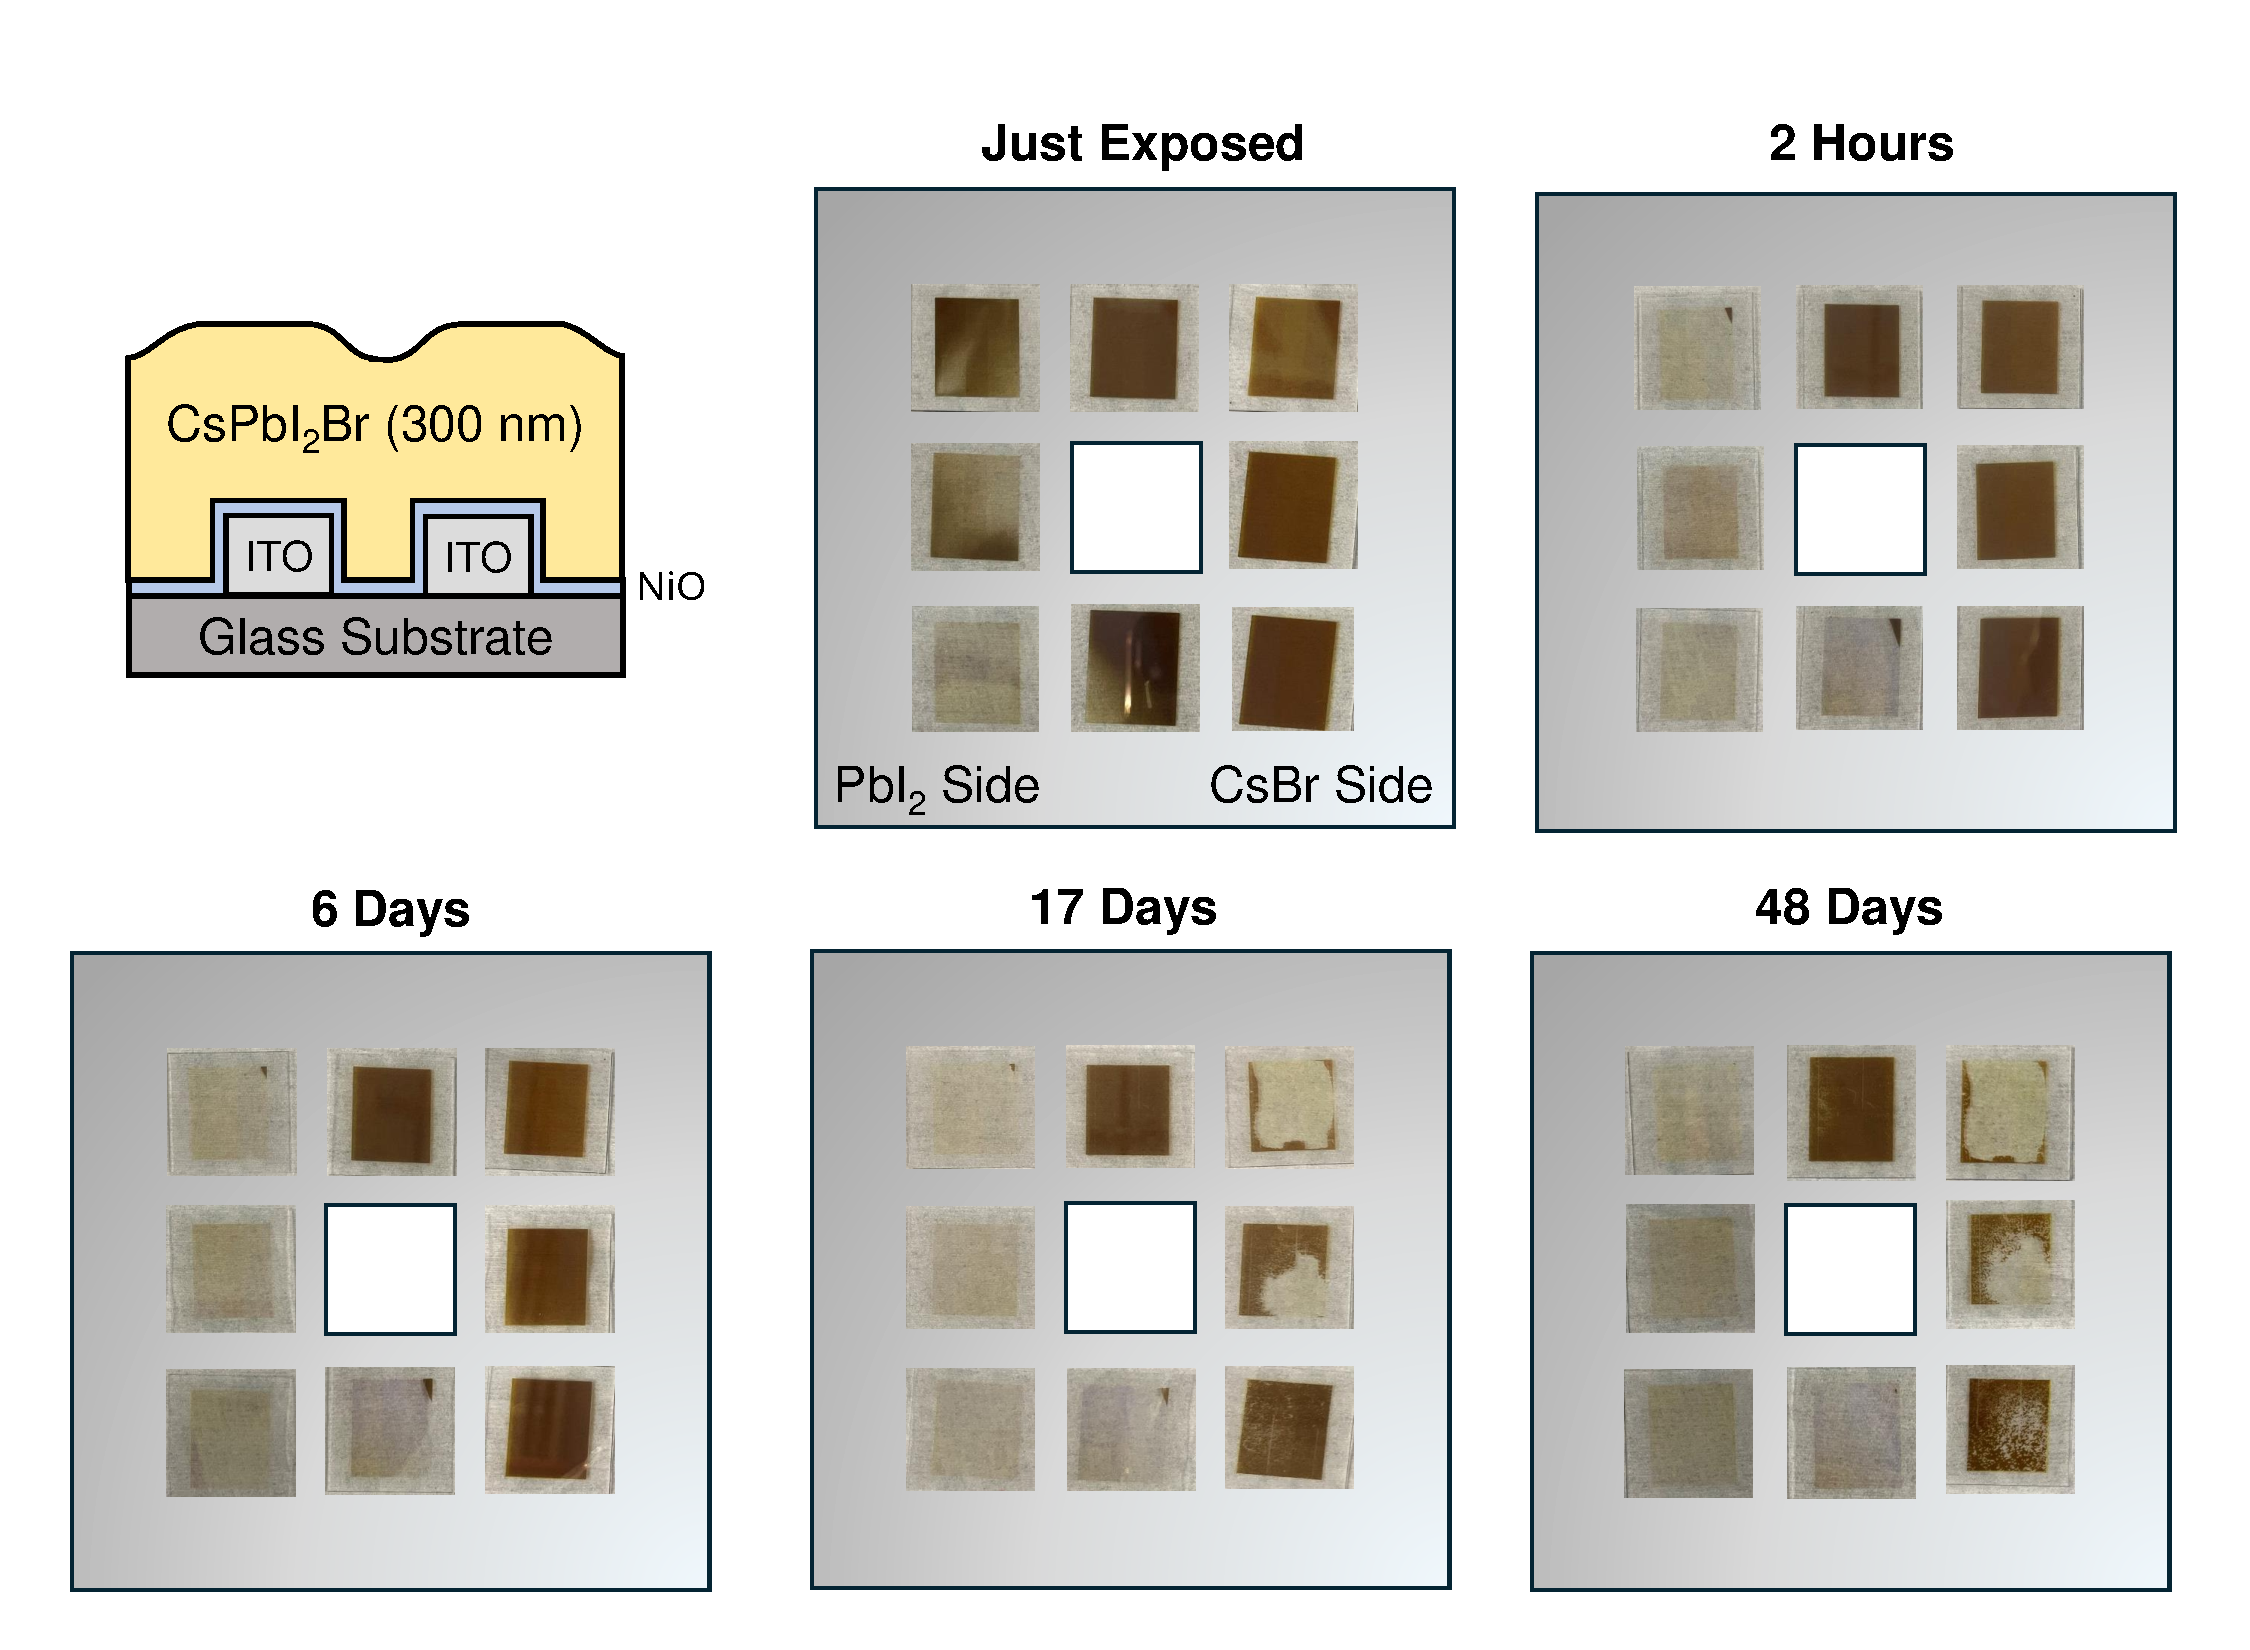
\includegraphics[width=\textwidth]{chapters/appendixB/images/Stability_No_Rotation_275_on_nio_repeated.pdf} % Replace with your image file
             
    \end{subfigure}

    \caption{Repetition of samples of glass - NiO}
    \label{fig:appendix:stability_on_NiO_v2}
\end{figure}

%%%%%%%%%%%%%%%%%%%%%%%%%%%%%%%%%%%%%%%%%%%%%%%%%%
% Keep the following \cleardoublepage at the end of this file, 
% otherwise \includeonly includes empty pages.
\cleardoublepage

% vim: tw=70 nocindent expandtab foldmethod=marker foldmarker={{{}{,}{}}}
